\documentclass[12pt]{article}
\usepackage{fontspec}

\setmainfont{Times New Roman} % Times New Roman, Arial, Calibri

\usepackage{setspace}
\setstretch{1.15}

\usepackage{pdflscape}

\usepackage{longtable}

\usepackage{graphicx}
\usepackage{float}
\usepackage{placeins}
\usepackage[backend=biber, style=numeric, sorting=none]{biblatex}
\addbibresource{references.bib}

\usepackage{geometry}
\geometry{top=2.5cm, bottom=2.5cm, left=2.5cm, right=2.5cm}

\usepackage{pdfpages}

\usepackage{listings}
\usepackage{xcolor}
% Define colors
\definecolor{codegreen}{rgb}{0,0.6,0}
\definecolor{codegray}{rgb}{0.5,0.5,0.5}
\definecolor{codepurple}{rgb}{0.58,0,0.82}
\definecolor{backcolour}{rgb}{0.95,0.95,0.92}

% Setup the listings package
\lstdefinestyle{mystyle}{
    backgroundcolor=\color{backcolour},
    commentstyle=\color{codegreen},
    keywordstyle=\color{magenta},
    numberstyle=\tiny\color{codegray},
    stringstyle=\color{codepurple},
    basicstyle=\ttfamily\footnotesize,
    breakatwhitespace=false,
    breaklines=true,
    captionpos=b,
    keepspaces=true,
    numbers=left,
    numbersep=5pt,
    showspaces=false,
    showstringspaces=false,
    showtabs=false,
    tabsize=2
}

\lstset{style=mystyle}

\usepackage{amsmath} % For mathematical features

\renewcommand{\theequation}{\thesection.\arabic{equation}}
\renewcommand{\thefigure}{\thesection.\arabic{figure}}

\usepackage{nomencl}
\usepackage{chngcntr}
\usepackage{amssymb}
\counterwithin{figure}{section}
\counterwithin{equation}{section}

\title{Identifying Dynamic Systems with Probabilistic Numerics}
\author{Harvey Walton}
\date{\today}

%Repeated Text
\newcommand{\ndiFigCaption}[1]{The rectangle method for finding the #1 bound of the integral of the standard Gaussian (normal) distribution between -2 and 1.}

\hyphenpenalty=700
\exhyphenpenalty=700

\makenomenclature

% Define nomenclature groupings
\renewcommand{\nomgroup}[1]{%
    \ifthenelse{\equal{#1}{G}}{\item[\textbf{Greek Symbols}]}{%
        \ifthenelse{\equal{#1}{L}}{\item[\textbf{Latin Symbols}]}{}}}

\setlength{\nomlabelwidth}{2cm}
%\renewcommand{\nomlabel}[1]{\textbf{#1}\hfil} % Bold the symbols and right-align
%\setlength{\nomitemsep}{-\parsep} % Reduce the space between items

\begin{document}
    \pagenumbering{roman}

    \thispagestyle{empty}
    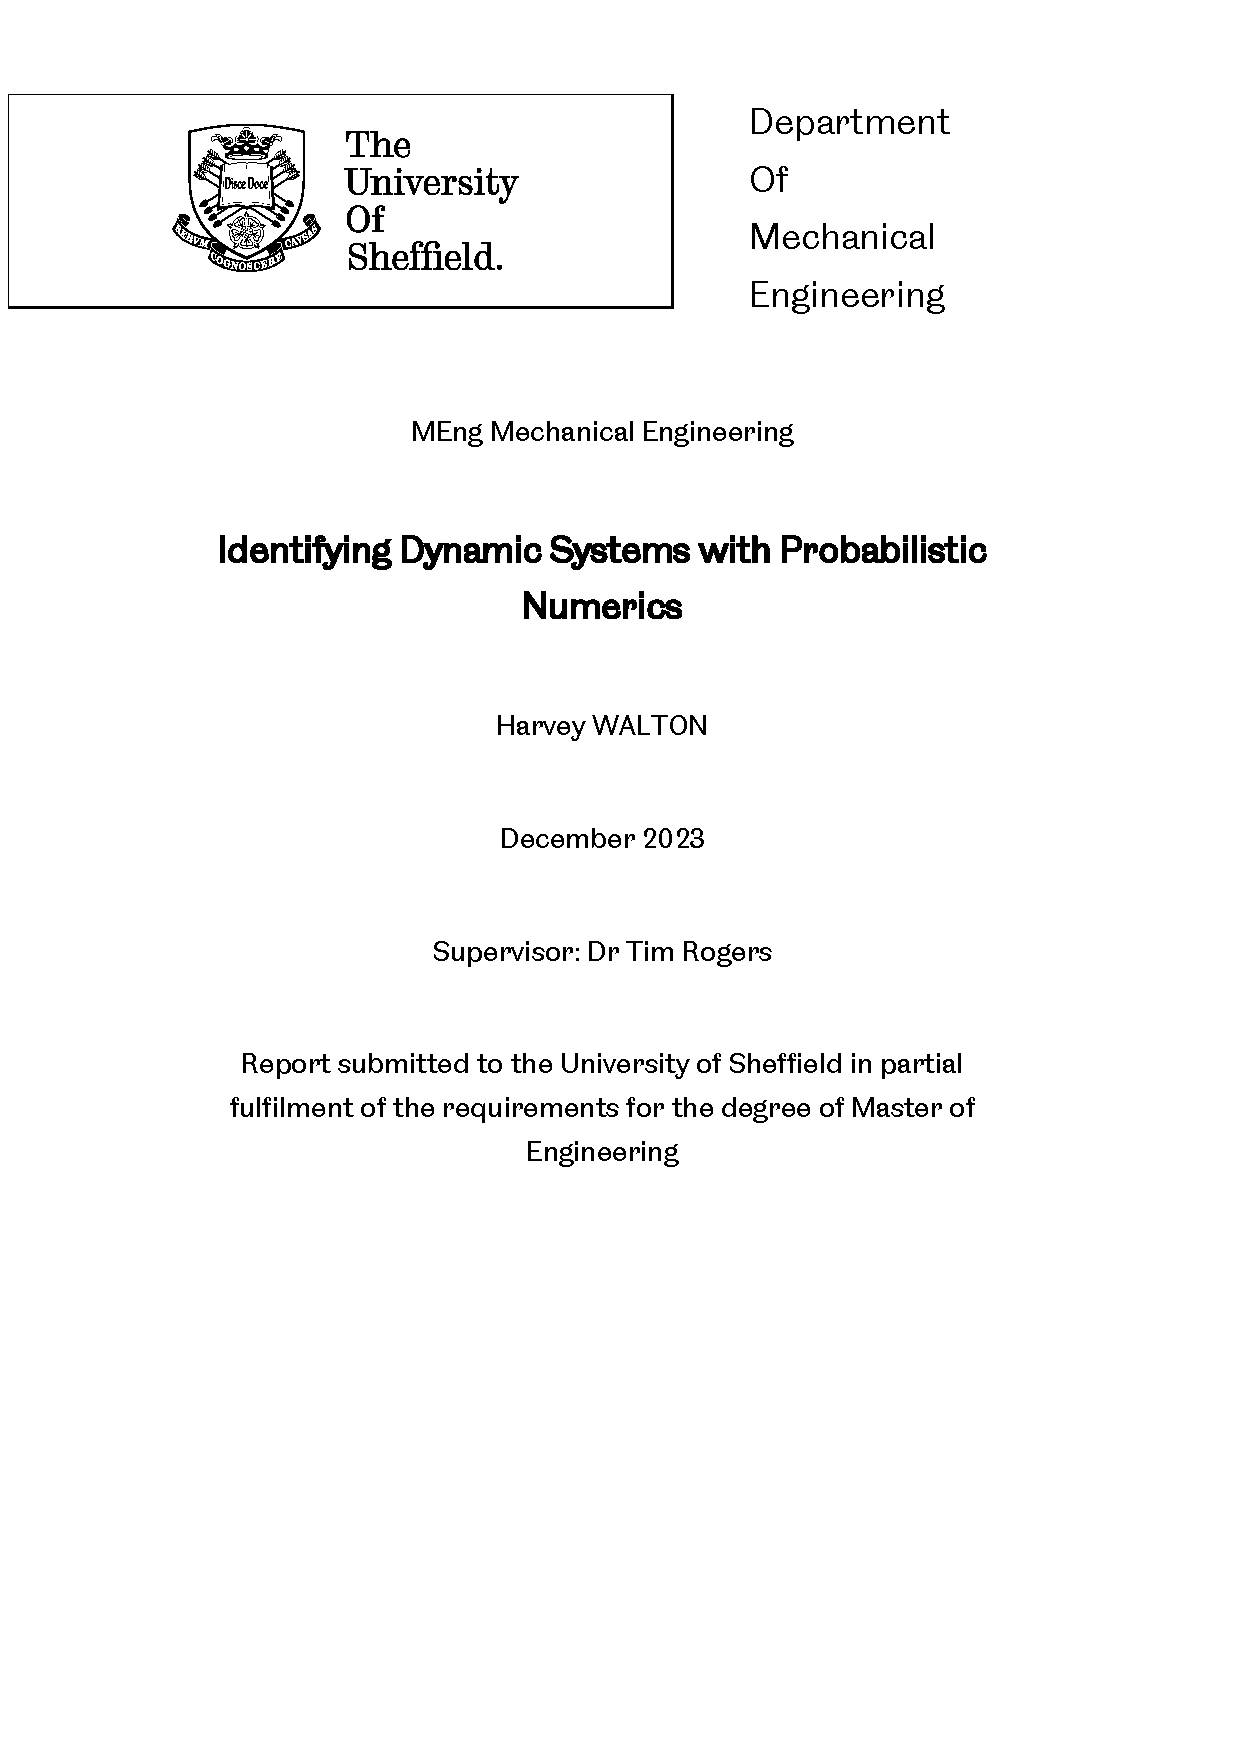
\includepdf[pages=1, frame, scale=1.09, pagecommand={}, offset=0 -35]{figures/titlepage.pdf}

    \printnomenclature

    \newpage
    \tableofcontents
    \newpage

    \pagenumbering{arabic}

    \section{Background and Understanding of the Problem}

    \subsection{Dynamic Systems}
    In the field of engineering, dynamics is focused on analyzing how systems, including structures and fluids, change and move.
    This dynamic behaviour is typically in response to a dynamic force that changes over time, such as aerodynamic forces or impacts from waves or bumps in the road.
    Studying dynamics is valuable because it has the potential to help prevent excessive vibration or oscillation of machinery, which is known to reduce the service life and in extreme cases can lead to catastrophic failure.
    Therefore, if it was possible to describe and more accurately predict the behaviour of systems and structures in response to the dynamic forces that are present in these systems, they could be designed to be perform better, be safer, and to have lower maintenance costs.
    However, the field of dynamics is far from being mastered, and there are still a large number of problems that cannot yet be solved.
    To begin, here are some examples of dynamic systems to illustrate why studying them is valuable:
    \begin{enumerate}
        \item A motorcycle suspension system is a combination of springs, dampers and linkages that connect the motorcycle chassis to its wheels.
        Its primary purpose is to keep the tyres in contact with the ground and without proper suspension, the tyres would lose traction when encountering bumps, especially when braking, accelerating or cornering [1].
        It is designed to allow some relative motion between the two in order to absorb impacts while at the same time trying to maintain its equilibrium position, and its equilibrium velocity of zero - both relative to the chassis.
        The dampers in the suspension produces a force proportional to the velocity, typically through viscous dampers.
        Think of these like syringes full of a liquid; the faster you move the plunger, the harder you have to push to maintain that velocity due to resistance to the flow caused by viscous drag forces.
        Similarly, damping in the system produces a force proportional to the velocity that acts to slow the wheel down and can be optimised by bringing the system back to equilibrium after a disturbance as fast as possible so that it is ready for the next bump (known as ``critical damping'').
        Too little damping, and the wheel will overshoot and oscillate back and forth before reaching equilibrium.
        Too much damping, and the wheel will not oscillate, but it will reach equilibrium more slowly than what is possible.
        Similarly, the spring creates stiffness in the system that produces a force with a magnitude proportional to the displacement of wheel from its equilibrium position which acts to return the wheel to this equilibrium position.
        The ideal balance between comfort and handling can be tailored to the specific use of the bike by setting the stiffness of the spring low enough that the system has time to absorb the impact softly, but high enough that the bike's responses to steering inputs are fast and reactive.
        Therefore, studying dynamic systems such as this one would be valuable because if it was possible to reliably predict how it will behave for different system parameters such as mass, stiffness and damping, it would be possible to design the system with the best system parameters within the given constraints in order to optimise the performance of the motorcycle for its purpose.

        \item An offshore wind turbine experiences a relentless random forcing the waves that repeatedly crash against the base of its tower.
        High cycle fatigue a phenomenon that causes cracks to grow over time from micro-defects in a structure due to cyclic loading below the elastic limit of the material.
        The rate at which this occurs increases with the amplitude of the stresses in the structure, which in turn increase with the amplitude of oscillation in response to this cyclic loading.
        If a periodic force is applied to a system with a specific frequency known as a resonant frequency, the amplitude of the oscillation may be large even for a small amplitude force, leading to a reduced lifespan from an excessive rate of high cycle fatigue.
        The same can happen in this case with a random force that has an \textit{average} frequency similar to the resonant frequency.
        Furthermore, the stresses could become so large that they exceed the ultimate tensile strength of the material, causing a sudden mechanical failure and the collapse of the turbine.
        Therefore, to make structures safer and reduce maintenance costs, it would be valuable to be able to model their behaviour in terms of dynamic properties such as this resonant frequency from system parameters such as the stiffness of the tower so that the frequencies at which they occur can be designed away from the expected frequencies of the periodic forces.

        \item An aircraft wing bends in response to aerodynamic forces.
        However, in this case the forces themselves change as the wing twists and bends.
        The interdependence of these two effects creates complicated ``nonlinear'' interactions that are difficult to model accurately.
        However, it is important to do so because if at high airspeed, energy from the wing forcing is added to the system faster than it can be dissipated, the positive feedback loop can lead to a phenomenon called aerodynamic flutter where the oscillations become larger and larger until they cause catastrophic failure.
    \end{enumerate}

    \subsection{Identifying Dynamic Systems}

    Dynamic systems have system parameters, which are fundamental characteristics of the system such as the aforementioned mass, stiffness and damping.
    ``Forwards modelling'' is when the observable behaviour of the system, known as the system properties are predicted from the system parameters using physical laws.
    These properties include the resonant frequencies, which are the forcing frequencies that produce a peak in amplitude of excitation, and mode shapes are the patterns of vibration at each resonant frequency, typically in the context of multi-degree-of-freedom (MDOF) systems.
    These MDOF systems are modelled as more than one point masses, and typically connected to each other and the environment by springs and dampers.

    Often a distinction is made between linear and nonlinear systems.
    Only linear systems comply with the principle of superposition, which states that ``when two or more waves simultaneously pass through a point, the disturbance at the point is given by the sum of the disturbances each wave would produce in absence of the other waves''~\cite{StudyComSuperposition}.
    This means that if you double the input force over time, the response over time is exactly the same, except that the displacement at any point in time will be double.
    This is not the case for nonlinear systems (such as the aircraft wing in the example above) where non-compliance with the principle of superposition causes the system parameters to distort as the magnitude of the input force is increased.
    This causes the response to become highly complex and chaotic, meaning that it is highly sensitive to initial conditions.
    Nonlinearity can even lead to bifurcations, which is where the system can exhibit one of multiple stable responses, or limit cycles, at a given frequency.
    Therefore, forward modelling is currently too difficult for systems that are non-linear.

    Unfortunately, in real life, everything is non-linear, and therefore forward modelling cannot currently be used to solve system properties exactly using the system parameters as an input.
    Only in rare cases are systems close enough linear that they can be approximated as such.
    What's worse is that even if a model did exist to solve the system, it would be of no use because typically not even the system parameters are known to be able to input them into the model.
    This inherent complexity is the key reason why the field of dynamics has not been mastered, and it means that currently for medium to highly non-linear systems - which is almost all systems - all that can be done is to take real life data measurements from an existing system and identify the system properties and parameters that best fit the observed data.
    Identifying dynamic systems is known as inverse modelling, but even this process is fraught with issues.

    \subsection{Classically Quantifying Uncertainty with Error Bounds}
    Identifying system parameters using this inverse modelling approach results in values that are not exact, but have an uncertainty associated with them that comes from multiple sources.
    The first cause of this uncertainty is due to noise that is always present to some degree in the sampled data due to the measuring devices - typically accelerometers - that are used to capture the input and response to the system.
    Furthermore, even if the true input and response could be sampled exactly, the non-identifiability problem states that since there are multiple sets of system parameters that could give the same set of observed outputs, it's impossible to uniquely determine them.
    Similarly, many algorithms make use of mathematical objects (such as matrix pseudoinverses) which have multiple alternatives, the correct choice of which is arguable and not definitive.
    This lack of uniqueness is represented in outputted system parameters by having an uncertainty around their value and classically, this uncertainty is represented using error bounds.
    For example, the damping ratio of a mode could be calculated in this way to be $0.1 \pm 0.02$, which provides a range bounded by an upper and lower limit which the true value is expected to be within.


    \subsection{The Fourier Transform and the Frequency Response Function (FRF)}

    In inverse modelling of dynamic system analysis, any collected time series data is almost always converted into the frequency domain.
    This is because the physical meaning of the system properties have a clear visual interpretation in this domain. %elaborate + figure
    Specifically, the Frequency Response Function (FRF) is typically found, which is defined as the frequency domain response divided by the frequency domain input force.
    The transformation of these functions from the time domain to the frequency domain relies on a linear transformation called the Fourier Transform, $F(\omega)$, as defined in Equation~\ref{eq:ft})

    \begin{equation}
        F(\omega) = \int_{-\infty}^{\infty} f(t) e^{-i \omega t} \, dt\label{eq:ft}
    \end{equation}
    \nomenclature[L]{$F(\omega)$}{Fourier Transform of $f(t)$}
    \nomenclature[G]{$\omega$}{Angular frequency}


    \noindent where $\omega$ is the angular frequency.
    This is an extremely powerful analytical technique that is used widely in engineering.
    However, it can only be applied in its base form to a function that is continuous in the domain $-\infty \text{ to } \infty$, meaning that it has a value defined at every point in time.
    Although in the real world time passes continuously forever, the Fourier Transform of data sampled from the real world cannot be found by directly using the continuous Fourier Transform.
    This is because this data is recorded over a finite window, and because it is typically discrete meaning that it is recorded at specific points in time instead of any point a continuous domain.
    Classically, a numerical method called the Discrete Fourier Transform algorithm called the Fast Fourier Transform is used in this case.

    A numerical method is a discrete approximation of a transformation that cannot be solved using its exact mathematical definition because this would be either impossible or impractical.
    Typically, these are used when working with discrete data such as data sampled from real life.

    \subsection{The Fast Fourier Transform Algorithm}
    Although discovering this fast way to compute the Discrete Fourier Transform revolutionised many engineering disciplines such as structural health monitoring, image compression, signal processing, and control theory\cite{Byjus2023}, its implementation has a number of challenges that have to be carefully handled.
    Firstly, the FFT assumes the input signal is periodic, which can lead to a phenomenon called spectral leakage if the signal is not an exact multiple of the chosen window\cite{MathStackExchange2023}.
    This can cause sharp resonance peaks to be smoothed out in the output because energy that should be concentrated at a peak frequency is spread across a range of frequencies nearby.
    But most importantly, the FFT can be highly sensitive to noise in the data, meaning a small amount of noise can create large fluctuations in the shape of the frequency spectrum, masking the true underlying frequencies and modal properties\cite{MathStackExchange2023}.

    Classically, the uncertainty of parameters calculated downstream of this FFT could be quantified with error bounds by a sensitivity analysis.
    Here, the uncertainty of the input data would be estimated, perhaps from the resolution of the measuring equipment, or by observation of the time domain sample data.
    Then, the upper and lower bounds of the system parameters could be estimated using the upper and lower bounds of the input data.
    However, this is not straightforward and typically requires additional techniques and considerations beyond the core algorithm.
    Furthermore, this process would not improve the poor robustness to noise of this FFT, only serve to quantify it.

    \subsection{Identifying Dynamic Systems with Probabilistic Numerics}
    This paper proposes a new method of performing the Fourier Transform and other linear transformations.
    This new method makes use of a machine learning model called a Gaussian Process (GP) which allows a continuous signal to be reconstructed from discrete sample data over a finite time interval.
    Moreover, it is defined in the continuous domain $-\infty \text{ to } \infty$ which means that the noise resilience of an FRF computed using this method may be improved because this can be transformed by the continuous Fourier Transform instead of resorting to the discrete FFT which is highly sensitive to noise.

    The outputs of the reconstructed function that this GP generate are probabilistic which means that the output is not itself a single point, but a Gaussian probability distribution defined by a mean and standard deviation.
    The GP model can be designed to include a noise term that explicitly models the observational noise.
    This gives the GP a way to distinguish between the signal and noise components, which may allow for Fourier Transform to be performed with better robustness to noise through its use of probabilistic numerics.

    \subsection{Implications of the Findings}

    \subsubsection{Implications in the Context of the Fourier Transform}

    A Fourier Transform method that can be applied to discrete data and that is more robust to noise than the FFT would have significant implications in various fields of engineering.

    In the context of modal analysis, the modal properties could be identified more precisely especially for nonlinear systems, whose complex dynamic behaviours can be obscured by noise.
    For example, noises may cause two closely spaced resonant frequencies to be mistaken for a single resonant frequency.
    Furthermore, better modelling and identification of nonlinear behaviour would allow earlier detection of changes in structural integrity in the context of Structural Health Monitoring because new or changes to nonlinear behaviour are typical of the formation or growth cracks or other defects.
    This in turn would allow engineers to make and maintain structures more safely being more likely to detect structural damage before catastrophic failure occurs.

    A Fourier Transform that is more robust to noise would improve other areas of engineering where it is used extensively such as signal processing, image processing and acoustic engineering.
    In these contexts, the Fourier Transform is used to simplify a computationally expensive operation called convolution into a simple pointwise multiplication in the frequency domain and so would enhance operations like signal filtering, image edge detection and acoustic noise reduction by reducing the distortion that occurs during these operations due to the presence of noise in the input data.


    More generally in engineering, this alternative method could be employed where numerical methods would classically need to be implemented to transform discrete data.
    Here, the same advantages of noise resilience provided by quantifying uncertainty with probabilistic numerics would apply.

    \subsection{The Gaussian Process Model}
    The Gaussian Process (GP) is being used to map a continuous ``latent'' function, $f(x)$, to our noisy discrete sampled data that takes an input $x$ (in this case, time) and outputs in a force.\nomenclature[L]{$f(x)$}{Latent function of the variable $x$}
    A Gaussian Process ``is a collection of random variables, any finite number of which have a joint Gaussian distribution''~\cite{rasmussen2006gaussian}.
    This is a distribution of a set of variables that include both our training data and points of interest on our latent function.
    It describes how the probability distribution of each variable depends on the values of the other variables.
    Assuming a mean of the latent function of zero, and a noisy observed force, $y_n = f(x_n)+\epsilon_n$, where $\epsilon_n \sim \mathcal{N}(0, \sigma^2_y)$, the joint density of the observed data and the latent, noise-free function on our test points is given~\cite{murphy2023probabilistic} by Equation~\ref{eq:joint-distribution}

    \begin{equation}
        \begin{pmatrix}
            \mathbf{y} \\
            \mathbf{f}^*
        \end{pmatrix}
        \sim \mathcal{N} \left(
        \begin{pmatrix}
            \boldsymbol{\mu}_X \\
            \boldsymbol{\mu}_*
        \end{pmatrix},
        \begin{pmatrix}
            \mathbf{K}_{X,X} + \sigma^2_y \mathbf{I} & \mathbf{K}_{X,*} \\
            \mathbf{K}_{X,*}^T & \mathbf{K}_{*,*}
        \end{pmatrix}
        \right)\label{eq:joint-distribution}
    \end{equation}

    \nomenclature[L]{$y_n$}{Noisy observed output based on the latent function, $f(x)$}
    \nomenclature[L]{$\mathbf{y}$}{A vector of $y_n$ values from a set of training points}
    \nomenclature[L]{$\mathbf{f}^*$}{A vector of values of the latent function evaluated at a set of test points, $\mathbf{X}_*$}
    \nomenclature[L]{$\mathbf{I}$}{Identity matrix}
    \nomenclature[L]{$\mathbf{K}_{X,X}$}{Covariance matrix for training input data, $\mathbf{K}(\mathbf{X},\mathbf{X})$}
    \nomenclature[L]{$\mathbf{K}_{X,*}$}{Covariance matrix between training inputs and test inputs, $\mathbf{K}(\mathbf{X},\mathbf{X}_*)$}
    \nomenclature[L]{$\mathbf{K}_{*,*}$}{Covariance matrix for test inputs, $\mathbf{K}(\mathbf{X}_*,\mathbf{X}_*)$}
    \nomenclature[G]{$\epsilon_n$}{Noise in observation, normally distributed with a mean of zero and a variance of $\sigma^2_y$}
    \nomenclature[G]{$\boldsymbol{\mu}_X$}{Mean of the Gaussian Process, given the training data $\mathbf{X}$}
    \nomenclature[G]{$\boldsymbol{\mu}_*$}{Mean of the Gaussian Process, given the test data $\mathbf{X}_*$}
    \nomenclature[G]{$\sigma^2_y$}{Variance of observation noise}


    \noindent where $\mathbf{y}$ is a vector of $y_n$ values from a set of training points, $\boldsymbol{\mu}_X$ is the mean of the Gaussian Process, given the training data $\mathbf{X}$, $\boldsymbol{\mu}_*$ is the mean of the Gaussian Process, given the test data $\mathbf{X}_*$, $\mathbf{f}^*$ is a vector of values of the latent function evaluated at a set of test points $\mathbf{X}_*$, $\mathbf{I}$ is the identity matrix and $\mathbf{K}_{X,X}$, $\mathbf{K}_{X,*}$ \& $\mathbf{K}_{*,*}$ are a type of covariance matrix, $\mathbf{K}(\mathbf{A},\mathbf{B})$, based on the ``kernel'' function, $k(a,b)$, when evaluated for each pair elements in the vectors $(\mathbf{X},\mathbf{X})$, $(\mathbf{X},\mathbf{X}_*)$ and $(\mathbf{X}_*,\mathbf{X}_*)$ respectively.
    Note that block matrix notation is used where matrices are conjoined to form a larger block matrix. \nomenclature[L]{$\mathbf{K}_{\mathbf{A},\mathbf{B}}$}{Covariance matrix of the kernel function, $k(a,b)$, evaluated for each pair of elements a, b in vectors $\mathbf{A}$, $\mathbf{B}$}\nomenclature[L]{$k(a,b)$}{Kernel function of arbitrary points, $a$, and $b$}

    The kernel is a special function that when input with two vectors, produces a covariance matrix that measures the similarity between each pair of inputs based on a set of hyperparameters.
    The function is chosen to reflect any prior knowledge about the problem domain, and must ensure that the resulting matrix is symmetrical about the main diagonal, and have a property called Positive Semi-definiteness.
    These hyperparameters need to be optimised by minimizing the Negative Log Marginal Likelihood (NLML), as defined~\cite{murphy2023probabilistic} in Equation~\ref{eq:NLML}

    \begin{equation}
        -\log p(\mathbf{D}|\boldsymbol{\theta}) = \frac{1}{2} (\mathbf{y} - \boldsymbol{\mu}_X)^T \mathbf{K}_{\sigma}^{-1} (\mathbf{y} - \boldsymbol{\mu}_X) + \frac{1}{2} \log |\mathbf{K}_{\sigma}| + \frac{N}{2} \log(2\pi)\label{eq:NLML}
    \end{equation}

    \nomenclature[L]{$\mathbf{D}$}{Training data}
    \nomenclature[G]{$\boldsymbol{\theta}$}{Set of hyperparameters}
    \nomenclature[L]{$\mathbf{K}_{\sigma}$}{Covariance matrix with noise term, $\mathbf{K}_{X,X} + \sigma^2_y \mathbf{I}$}
    \nomenclature[L]{$N$}{Number of training points}

    \noindent where $\mathbf{D}$ is the training data, $N$ is the number of training points, $\boldsymbol{\theta}$ is the set of hyperparameters and $\mathbf{K}_{\sigma} = \mathbf{K}_{X,X} + \sigma^2_y \mathbf{I}$ is the covariance matrix with the noise term.
    This measures how well the model explains the observed data for a given set of hyperparameters while penalizing complexity to avoid overfitting, which is when the model fits the training data so well that it generalises poorly to new test data.
    By minimizing this NLML, we identify the hyperparameter values that are most likely to produce the observed training data.


    By a process called conditioning the joint Gaussian prior distribution on the observations~\cite{rasmussen2006gaussian}, the ``posterior'', or prediction of the latent function when evaluated at a test point given our set of sampled training points~\cite{murphy2023probabilistic} can be found, as shown in Equation~\ref{eq:18.51}, where $\boldsymbol{\mu}_{*\vert \mathbf{X}}$ and $\boldsymbol{\Sigma}_{*\vert \mathbf{X}}$ are the conditional mean and covariance of the GP, given the training data, given in Equation~\ref{eq:18.52} and Equation~\ref{eq:18.53} respectively.

    \begin{equation}
        p(\mathbf{f}^* \vert \mathbf{D}, \mathbf{X}^*) = \mathcal{N}(\mathbf{f}^* \vert \boldsymbol{\mu}_{*\vert \mathbf{X}}, \boldsymbol{\Sigma}_{*\vert \mathbf{X}})\label{eq:18.51}
    \end{equation}

    \begin{equation}
        \boldsymbol{\mu}_{*\vert \mathbf{X}} = \boldsymbol{\mu}_* + \mathbf{K}_{X,*}^T (\mathbf{K}_{X,X} + \sigma^2_y \mathbf{I})^{-1} (\mathbf{y} - \boldsymbol{\mu}_X)\label{eq:18.52}
    \end{equation}

    \begin{equation}
        \boldsymbol{\Sigma}_{*\vert \mathbf{X}} = \mathbf{K}_{*,*} - \mathbf{K}_{X,*}^T (\mathbf{K}_{X,X} + \sigma^2_y \mathbf{I})^{-1} \mathbf{K}_{X,*}\label{eq:18.53}
    \end{equation}

    \nomenclature[G]{$\boldsymbol{\mu}_{*\vert \mathbf{X}}$}{Conditional mean of the Gaussian Process, given the training data}
    \nomenclature[G]{$\boldsymbol{\Sigma}_{*\vert \mathbf{X}}$}{Conditional covariance of the Gaussian Process, given the training data}

    This GP is closed under the action of linear operators which means that it can be described using only a combination of operations that comply with the principle of superposition.
    Incredibly, since the Fourier Transform is also a linear transformation, the result of this transformation of the GP is yet another GP\@.
    Therefore, modelling uncertainty with probabilistic numerics allows this uncertainty information to be transferred from the time domain to the frequency domain.


    \section{Aims and Objectives}
    \subsection{Aim}
    To improve the noise resilience of time series data when converted to frequency domain.

    \subsection{Objectives}
    The overarching aim can be broken down into four objectives:
        \begin{enumerate}
            \item Get a working Gaussian Process model.
            This involves:
                \begin{itemize}
                    \item Choosing and creating a Kernel.
                    \item Implementing optimisation of Kernel hyperparameters. \label{item:nll}
                    \item Creating a prediction function to predict the outputs of new inputs. \label{item:predict}
                \end{itemize}
            \item Scale to Large data by implementing a Sparse GP approximation.
            \item Adjust this model to enable the closed form Fourier Transform to be found.
            \item Compare the noise resilience with existing Discrete Fourier Transform methods such as the Fast Fourier Transform.\label{noise-resiliance}
            \item Stretch Objective: Compare the smoothing out of sharp resonance peaks due to spectral leakage.\label{stretch-obj}
        \end{enumerate}

    \section{Work Completed to Date}
    The first thing needed to be complete was the basic Gaussian Proces.
    This was implemented using the programming language Python and consisted of the following components:
    \subsection{The Data}
    Previously collected turbine tap test data~\cite{MEC326} was converted to a .csv file (a file that formats data into table of values), and imported into python.
    The tap data consisted of accelerometer data from the tip of a hammer as well as a single location on a turbine blade when struck at 10 positions.
    This was sampled at a rate of $16,384 Hz$ for just under 4 seconds.
    For simplicity, only the response data the first position was imported, and a small set of 100 samples was selected from the centre (to reduce computation time initially).
    This time series data, as shown in the ``Force Response'' plot in Figure~\ref{fig:input-response-plot}, was used as training data to be fit by the GP\@.

    \begin{figure}[ht]
        \centering
        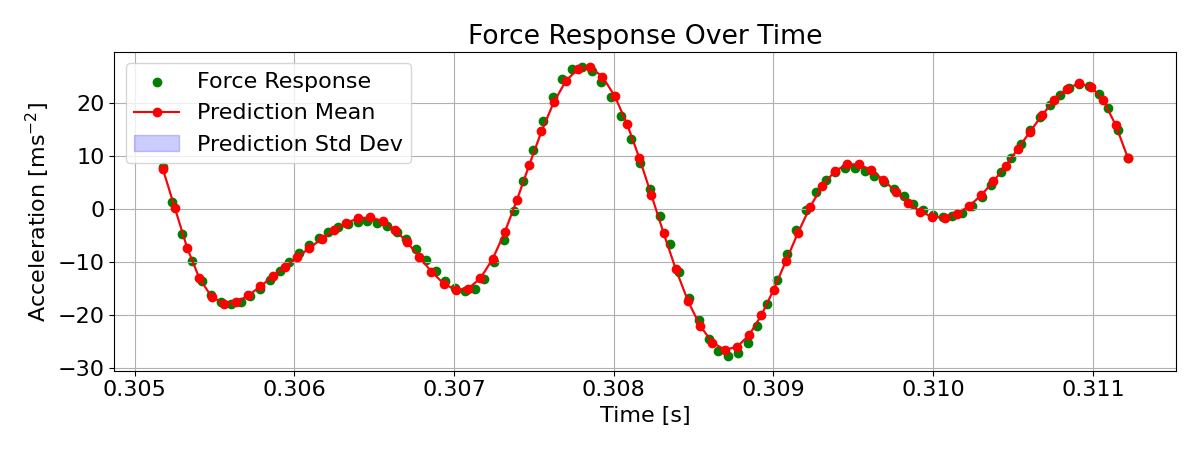
\includegraphics[width=1.0\linewidth]{figures/input-response-plot/input-response-plot.png}
        \caption{The time series data, and the mean and standard deviation of the GPs prediction of it. Note that the prediction functions of mean and standard deviation that are output by the Gaussian Process are infact continuous, but must be evaluated at a discrete set of points in order to be plotted}
        \label{fig:input-response-plot}
    \end{figure}



    \subsection{The Kernel}
    Next, a python class was created to contain the kernel.
    The Squared Exponential Kernel~\cite{duvenaud2014kernel}, defined in Equation~\ref{eq:se-kernel} was chosen to reflect the nature of the sample data that is continuous and smooth, with no sudden jumps.
    In addition, it only has two hyperparameters, this low number speeds up their optimisation process compared to alternative kernels.

    \begin{equation}
        \mathbf{K}_{ij} = \sigma^2 \exp\left(-\frac{(\mathbf{x}_i - \mathbf{x}_j)^2}{2l^2}\right) \label{eq:se-kernel}
    \end{equation}
    \nomenclature[L]{$\mathbf{K}_{ij}$}{Element of the covariance matrix, $\mathbf{K}$, at index $i, j$}
    \nomenclature[L]{$\mathbf{x}_i, \mathbf{x}_j$}{Input vectors}
    \nomenclature[L]{$\sigma^2$}{Variance, a hyperparamer in the context of the kernel}
    \nomenclature[L]{$l$}{Length scale parameter of the SE kernel}

    \noindent where $\mathbf{K}_{ij}$ is the element of the covariance matrix, $\mathbf{K}$, at index $i, j$, $\mathbf{x}_i, \mathbf{x}_j$ are input vectors, $\sigma^2$ is the variance hyperparameter, and $l$ is the length scale parameter of the SE kernel.

    The `variance' hyperparameter is a scale factor that determines the average distance of the function away from its mean, whereas the `length' hyperparameter determines how smooth or wiggly the function is, i.e., how fast the function can change direction.

    \subsection{Hyperparameter Optimisation}
    Next, this kernel class was added as an attribute to a class for the GP model itself.
    This allowed the kernel to be computed for different pairs of arrays as needed.
    This GP model also contained an algorithm to optimise the hyperparameters of the kernel by minimising the Negative Log Marginal Likelihood.
    It did this by multiplying each hyperparameter in turn by the exponent of a normally distributed continuous random variable.
    Imagine that only if the new NLML was lower than the previous, the hyperparameter was updated.
    If this was the case, the algorithm could get stuck in what is known as a local minimum, and never find the global minimum.
    This would be analogous to a ball that ``tried'' to find the bottom of a valley by always rolled directly downhill.
    If it got stuck in a small ditch half-way down the larger hill, it would never find the lowest point.
    Therefore, a mechanism was added to the algorithm to avoid this:
    If the new NLML was higher (i.e., worse) than the previous, the hyperparameter was maybe still updated, with a larger probability the closer the NLML was to the previous NLML.
    This enabled the algorithm to better find the global maximum because it was less likely to of get stuck in a local minima.

    \subsection{Predict Function}
    Next, the predict function was constructed, which accurately calculated the mean and standard deviation of the latent function as shown by the ``Prediction Mean'' and ``Prediction Std Dev'' plots in Figure~\ref{fig:input-response-plot}.
    Furthermore, when Gaussian noise was added to the input data, the standard deviation prediction becomes larger to take account for this noise as shown in Figure~\ref{fig:input-response-noise}.


    \begin{figure}[ht]
        \centering
        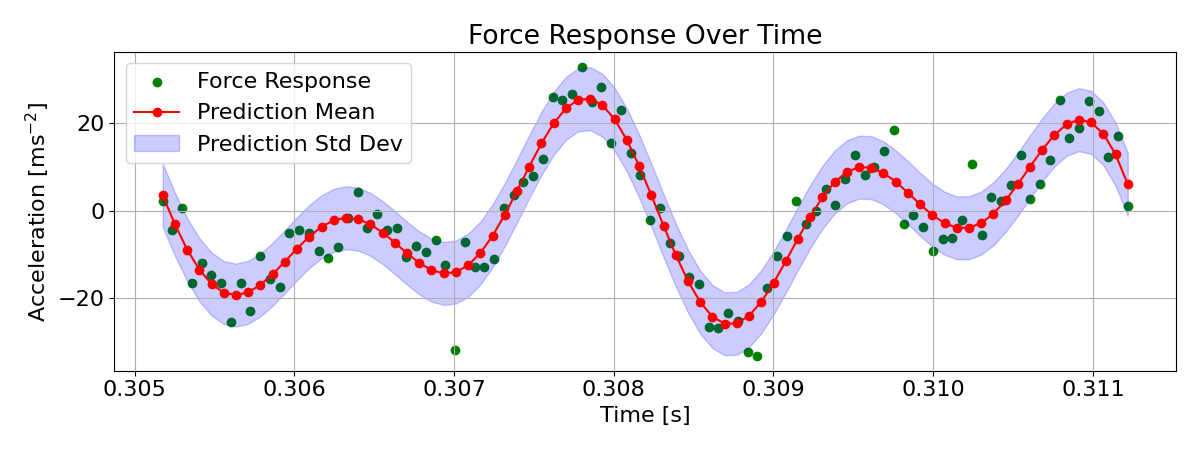
\includegraphics[width=1.0\linewidth]{figures/input-response-noise/input-response-noise.png}
        \caption{The prediction function fit by the GP overlayed on the training data. Note that the standard deviation of the prediction increases for data with more noise.}
        \label{fig:input-response-noise}
    \end{figure}

    \section{Plan for Future Work}
    Firstly, the Sparse GP approximation known as the Fully Independent Training Conditional (FITC) will be complete to allow the model to scale to large data~\cite{q-candela}.
    This will reduce the complexity of the training phase from $O(N^3)$ to $O(MN^2)$, where M is a set of inducing points chosen to be a subset of the original training points, evenly spaced, and $N \gg M$. \nomenclature[L]{$M$}{Number of inducing points in Sparse GP} \nomenclature[L]{$O()$}{Big O notation, used to describe the complexity - or ``order'' of an algorithm}
    This modification will be made to both the NLML and predict functions, which required a very specific implementation involving multiple mathematical tricks in order to keep the calculations numerically stable and efficient in terms of computation time and memory required.
    This is because certain matrix operations such as determinants and inversions can give imprecise results for large matrices containing floating point numbers, which is a format that computers use to store continuous variables as a decimal as opposed to integers type variables.
    After this is complete, the hyperparameters can be optimised and the GP can be fit for functions containing more than 1000 data points in a significantly reduced computation time.

    After the implementation of the Sparse GP, the next step will be to extend the input space of the joint Gaussian distribution to the frequency domain by incorporating the Fourier transform.

    Then, the best method to compare the robustness to noise of the Fourier transform computed using the GP model vs the classical FFT model needs to be determined (Objective~\ref{noise-resiliance}).
    One method of doing this uses the Mean Squared Error (MSE), which is a method of measuring the quality of an estimator (lower is better) by measuring the average of the squares of the differences between the points at each index position in the series, as shown in Equation~\ref{eq:mse}

    \begin{equation}
        \text{MSE} = \frac{1}{n} \sum_{i=1}^{n} (A_i - B_i)^2
        \label{eq:mse}
    \end{equation}

    \nomenclature[L]{$A_i$, $B_i$}{Values of vectors $\mathbf{A}$, $\mathbf{B}$ at index i}

    \noindent where $A_i$, $B_i$ are the values of vectors $\mathbf{A}$, $\mathbf{B}$ at index i:

    First the Fourier Transform can be computed using each method.
    Then, some Gaussian noise can be added to the data and the FRF can be computed again using both methods.
    Next, the (discrete) Mean Squared Error can be computed between Fourier Transforms of the unmodified and noisy data using the FFT method with a suitable setup of parameters such as window size and type.
    Similarly, the MSE can be computed between the mean functions of the Fourier Transforms of the unmodified and noisy data generated by the Gaussian Process method.
    Since these mean functions are continuous, they first need to be discretised at the same frequencies present in the FFTs generated by the first method.
    The two MSEs can then be used to make a comparison between robustness to noise, of each method.
    This could be repeated for different levels and types of noise (Gaussian vs white noise) to test how each method performs under various conditions.

    If time allows, the stretch objective (\ref{stretch-obj}) of comparing how smoothed out sharp resonance peaks are due to spectral leakage can be complete.
    To do this, the Fourier Transform of a pure sine wave should be found using both the GP and FFT methods.
    This is because it can be solved analytically on paper to provide a Fourier Transform with a sharp peak at the frequency of the wave, and the MSE of each method against the mathematically precise analytical solution can be compared.

    Finally, a conclusion can be drawn regarding the utility of the new Gaussian Process (GP) method of computing the Fourier Transform presented in this paper when compared to the classical Fast Fourier Transform (FFT) with respect to robustness to noise and prevention of artifacts due to spectral leakage.
    Since the addition of noise is an inherently random, this should be repeated several times and statistical techniques should be employed to show whether any differences in MSE are statistically significant.
    One such technique is hypothesis testing, which provides a framework to state whether there is sufficient evidence to reject the ``null'' hypothesis.
    This means that the default stance the new GP method is no better than classical methods is assumed unless there is sufficient evidence to prove otherwise beyond a reasonable doubt.

    \subsection{Future Work Time Plan}
    A Gantt chart outlining the main steps and the approximate schedule for the remaining work in the project is included in Figure~\ref{fig:gantt-chart_}:

    \begin{landscape}
        \begin{figure}[p] % 'p' places the figure on a page of its own
            \centering
            \includegraphics[width=\linewidth]{figures/gantt_chart/gantt-chart_.png}
            \caption{A Gantt chart showing work remaining, using a format modified from~\cite{DataCampGanttChart2021}. This includes scheduled delays in the Christmas and Easter holidays to allow for exam revision and as a buffer to catch up to the schedule if the project is falling behind}
            \label{fig:gantt-chart_}
        \end{figure}
    \end{landscape}

%    \appendix
\section{The use of generative AI (ChatGPT)}
OpenAI's ChatGPT interface, powered by the GPT-4 large language model, was used to implement the Negative Log Marginal Likelihood (NLML) method in my code in a specific way to ensure numerical stability though the use of the ``Cholesky decomposition''.
The prompt and output is provided in Figure~\ref{fig:chat-NLML}.
\begin{figure}[htbp]
    \centering
    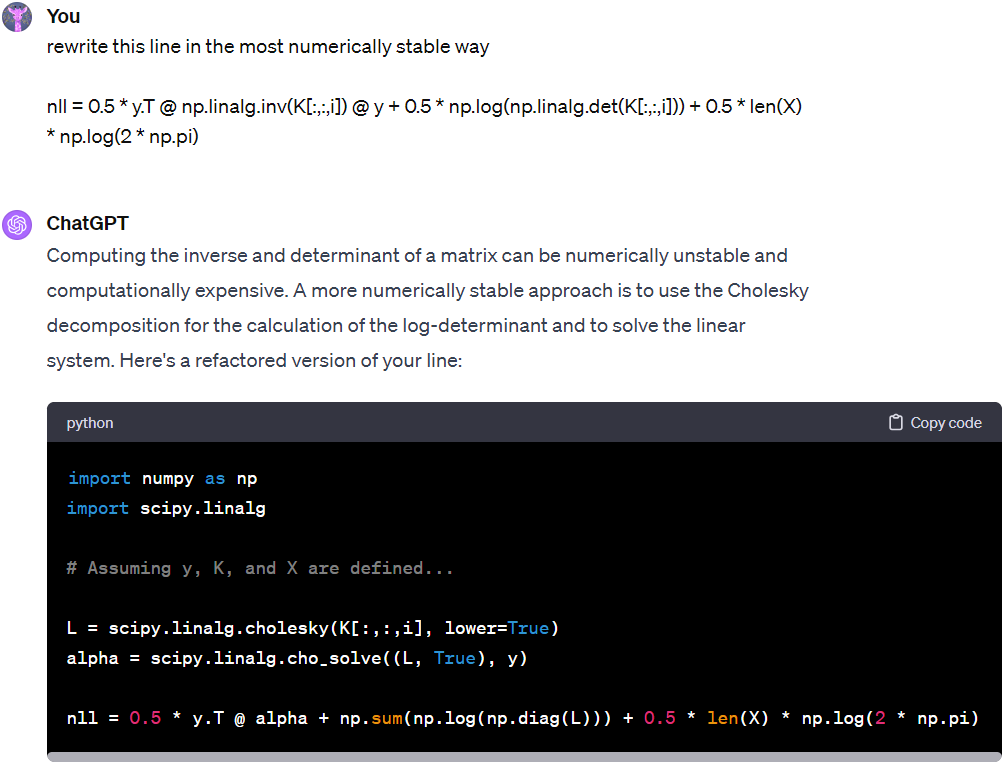
\includegraphics[width=1\linewidth]{figures/chat-NLML/chat-NLML.png}
    \caption{ChatGPT prompt and output providing a way to compute the NLML that is faster and more numerically stable}
    \label{fig:chat-NLML}
\end{figure}

\FloatBarrier

In order to ensure that this function was valid, its implementation was confirmed by the relevant literature~\cite{murphy2023probabilistic}~(Section 18.3.6).
After which, this function was simplified and adapted into that it could be to be added to the $gp\_model$ class as a method, and so that it would work with the way the input data was formatted, as shown in Listing~\ref{1st:NLML}

\begin{lstlisting}[caption={Method used to calculate the Negative Log Marginal Likelihood (NLML).} language=Python,label={lst:NLML}]
    def compute_nlml(self, hyperparameters):
    self.update_hyperparameters_and_debug(hyperparameters)
    self.reshape_X_and_y()

    if self.gp_algo == 'cholesky':
        K = self.gp_kernel.compute_kernel(self.X, self.X)
        K += np.repeat(np.array(np.eye(len(self.X)) * 1e-3)[:,:, np.newaxis], self.X.shape[1], axis=2)
        debug_K = np.squeeze(K)
        L = scipy.linalg.cholesky(K[:, :, 0], lower=True)
        n = len(self.y)
        one_vector = np.ones(n)
        y_adj = self.y - self.y_mean

        alpha = scipy.linalg.cho_solve((L, True), y_adj)

        term_1_c = (0.5 * y_adj.T @ alpha).item()
        term_2_c = np.sum(np.log(np.diag(L)))
        term_3_c = 0.5 * n * np.log(2 * np.pi)

        nlml = term_1_c + term_2_c + term_3_c

        out_c = {
            'nlml': nlml,
            'term_1': term_1_c,
            'term_2': term_2_c,
            'term_3': term_3_c
        }

        return out_c

\end{lstlisting}




    \printbibliography

\end{document}